\clearpage{\pagestyle{empty}\cleardoublepage}
\chapter{Tecnologie utilizzate}                %crea il capitolo
%%%%%%%%%%%%%%%%%%%%%%%%%%%%%%%%%%%%%%%%%imposta l'intestazione di pagina

\subsection{Angular}
\textbf{Angular} è un framework open source per lo sviluppo di applicazioni web scritto interamente in TypeScript.

Un elemento fondamentale per la costruzione di applicazioni Angular è il componente, al quale viene affidato il controllo di una porzione dello schermo, acquisendo la responsabilità di visualizzare i dati ricevuti e gestirne l’interazione con l’utente secondo il concetto di view.

Una moderna applicazione Angular è sintetizzabile in un insieme di componenti ordinate in modo gerarchico con le quali vengono fornite le funzionalità con cui far interagire l’utente.

Tra i principali motivi che rendono vantaggioso questo modello di programmazione vi è il fatto di poter assemblare applicazioni diverse utilizzando un insieme comune di componenti, favorendo quindi il riutilizzo del codice; al contempo la struttura definita dell’applicazione ne favorisce la suddivisione in moduli e la leggibilità del codice scritto.

\vspace{5mm}

Ogni componente ha un modello HTML che dichiara come quel componente viene visualizzato.

Angular estende l'HTML con una sintassi aggiuntiva che permette di inserire valori dinamici inizializzati nel componente. Angular aggiorna automaticamente il DOM renderizzato a ogni cambiamento dello stato del componente e seguendo le istruzioni fornite dalle cosiddette direttive. Questo modello di progettazione consente di scrivere codice più flessibile e testabile.

Angular inoltre fa uso del pattern dependency injection, che consente di dichiarare le dipendenze delle classi TypeScript lasciando gestire l'istanziazione interamente al framework. Quando Angular crea un componente, chiede all’injector i servizi richiesti. Un injector mantiene un container delle istanze dei servizi che sono stati precedentemente creati. Se un’istanza di un servizio richiesto non è nel container, l’injector ne crea uno e lo aggiunge al container.

\begin{figure}[H]
\centering
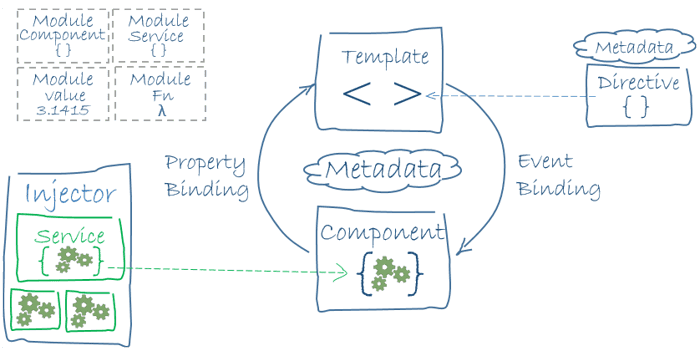
\includegraphics[scale=0.5]{res/angular.png}
\caption{Struttura di Angular}
\label{fig:angular}
\end{figure}

Per comunicare con i servizi di backend tramite HTTP, il servizio \texttt{HttpClient} usa observable e offre il metodo \
\texttt{HttpClient.get()} per recuperare i dati da un server. Il metodo asincrono invia una richiesta HTTP e restituisce come risposta un observable che emette i dati richiesti.

\subsubsection{Vantaggi e svantaggi}
Essendo basato su TypeScript, un linguaggio di programmazione che differisce da JavaScript e che offre numerose funzionalità aggiuntive come ad esempio la presenza di tipi statici, possono essere implementati numerosi tool per supportare meglio i programmatori e ridurre i bug nelle applicazioni.
Altra differenza importante è la presenza di numerose funzionalità aggiuntive come RxJS o la presenza stessa di un modello dei dati consistente integrato grazie al linguaggio Typescript, elemento assente ad esempio nel framework rivale React.

Al contempo l’onere di avere molte funzionalità integrate comporta un peso maggiore in termini di spazio di archiviazione in seguito alla prima installazione, mentre in altri concorrenti il peso effettivo del framework è decisamente inferiore, risultando
migliori per applicazioni meno complesse o che necessitano di meno funzionalità di quelle proposte da Angular.

Infine va rilevata una ridotta flessibilità del framework di Google rispetto ai rivali, con tutti i vantaggi e gli svantaggi derivanti da questa scelta soprattutto a livello progettuale. Un programmatore che sceglie Angular desidera una progettazione meno
impegnativa e approva tutte le scelte che il framework ha preso al posto suo; un programmatore di un altro framework desidera invece fare delle scelte personalizzate, dettate dalle proprie necessità progettuali, assumendosi poi però la responsabilità di mantenere aggiornate tutte le dipendenze inserite all’interno della propria applicazione.

\subsection{Bootstrap}
\textbf{Bootstrap} è un framework CSS gratuito e open source per la creazione di siti e applicazioni per il web. Contiene modelli di design basati su CSS e estensioni opzionali di JavaScript per tipografia, moduli, pulsanti, navigazione e altri componenti dell'interfaccia.

Tra le principali caratteristiche di questa libreria troviamo la piena compatibilità con tutte le ultime versioni di tutti i principali browser utilizzati, il supporto al responsive web design, l’adozione di una filosofia mobile-first per quanto riguarda il design oltre che un’ottima documentazione a corredo della libreria per rendere più facile la sua diffusione.

Gli sviluppatori possono sfruttare le classi CSS definite in Bootstrap per personalizzare ulteriormente l'aspetto dei loro contenuti.\cite{bootstrap}

\subsection{Node.js}
\textbf{Node.js} è un runtime JavaScript basato sugli eventi, non bloccante e asincrono costruito sul motore JavaScript V8 di Chrome e sulla libreria libuv. È usato per sviluppare applicazioni che fanno un ampio utilizzo di JavaScript sia lato client che lato server, e che quindi beneficiano della riciclabilità del codice e dell'assenza di commutazione di contesto.

Se un task entra in fase di stallo o pausa per l'esecuzione di un operazione I/O, può essere avviato un altro task. Ciò garantisce un alto tasso di efficienza, in quanto non è necessario attendere l'esecuzione di un singolo task per proseguire l'esecuzione dell'intero programma.

Per facilitare lo sviluppo di codice JavaScript complesso, Node.js supporta lo standard CommonJS che permette uno sviluppo modularizzato e la distribuzione di software in pacchetti attraverso Npm.\cite{stackoverflow-node.js}

Node.js usa un \code{[event loop][]} come costrutto di runtime anziché una libreria come in altri linguaggi. In altri sistemi, c'è sempre una chiamata bloccante per avviare l'event-loop. In genere il comportamento è definito tramite callback all'inizio di uno script e alla fine avvia un server attraverso una chiamata bloccante come EventMachine::run(). In Node.js non esiste alcuna chiamata per avviare il ciclo. Node.js entra semplicemente nel ciclo degli eventi dopo aver eseguito lo script di input, e ne esce quando non ci sono più callback da eseguire.\cite{node.js-about}

Quando Node.js viene avviato, inizializza l'event loop, processa gli script di input forniti che potrebbero effettuare chiamate API asincrone, programmare timer o chiamare \code{process.nextTick()}, per poi processare l'event loop.\cite{node.js-eventloop}

Le operazioni dell'event loop possono essere suddivise in fasi; ciascuna di esse ha una coda FIFO di callback da eseguire. Quando l'event loop entra in una fase, eseguirà qualsiasi operazione a essa relativa, per poi eseguire callback nella coda di quella fase finché non viene svuotata o quando è stato raggiunto il numero massimo consentito di callback eseguite, e quindi entrare nella fase successiva.\cite{node.js-eventloop}

\begin{figure}[h]
\begin{center}
  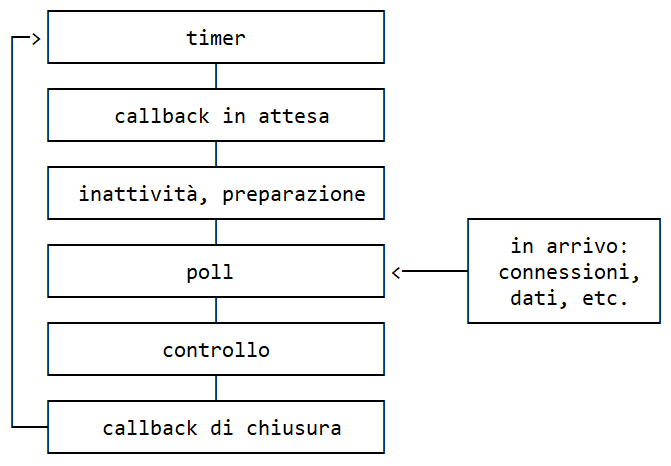
\includegraphics[width=0.8\linewidth]{res/EventLoop.png}
  \caption[Rappresentazione visuale delle transizioni delle fasi dell'event loop.]{Rappresentazione visuale delle transizioni delle fasi dell'event loop.\protect\cite{node.js-eventloop}}
  \label{fig:EventLoop}
\end{center}
\end{figure}

Le fasi dell'event loop sono le seguenti:
\begin{itemize}
\item \textbf{timer}: questa fase esegue le callback programmate da \code{setTimeout()} e \code{setInterval()}.
\item \textbf{callback in attesa}: esegue le callback di input/output prelevate dalla coda di attesa relative a operazioni di sistema, come ad esempio errori TCP.
\item \textbf{inattività, preperazione}: operazioni interne.
\item \textbf{poll}: vengono prelevati e inseriti nella coda nuovi eventi collegati al completamento di operazioni di I/O. Se la coda non è vuota, verranno processate le diverse callback in essa presenti. In caso contrario, se sono state registrate delle callback con la funzione \code{setImmediate()}, verrà terminata questa fase e si passerà alla fase successiva per processarle. Nel caso in cui non siano state registrate callback con la funzione \code{setImmediate()}, l'event loop resta in attesa che vengano aggiunte nuove callback alla coda. Mentre è in questa fase, l'event loop controlla se sono presenti callback che devono essere eseguite nella coda dei timer e, se lo sono, ritorna nella prima fase ed esegue le callback presenti in quella coda.\cite{mrwebmaster}
\item \textbf{controllo}: vengono invocate le callback \code{setImmediate()}.
\item \textbf{callback di chiusura}: vengono gestiti gli eventi di chiusura, per pulire lo stato dell'applicazione.
\end{itemize}

La funzione \code{process.nextTick()} viene eseguita subito dopo il completamento dell'operazione corrente, indipendentemente dalla fase in cui l'event loop si trova. È principalmente utilizzata per gestire errori, risorse non necessarie, ritentare richieste non andate a buon fine, oppure per effettuare operazioni dopo l'esaurimento dello stack delle chiamate ma prima che l'event loop continui.\cite{node.js-eventloop}

\subsection{Npm}
Il package manager \textbf{npm} è una raccolta di pacchetti gratuiti o a pagamento utilizzabili sul proprio progetto di sito web.
Utilizzabile al seguito dell’installazione di Node.js viene messo a disposizione come strumento da linea di comando con il quale scaricare moduli JavaScript poi disponibili all’interno del proprio progetto. Viene data la possibilità allo sviluppatore di caricare i propri moduli per metterli a disposizione della community.

\subsection{Express.js}
\textbf{Express.js} è un framework per applicazioni web Node.js flessibile e leggero che fornisce una serie di funzioni avanzate per applicazioni web e dispositivi mobili.

Permette di gestire le richieste HTTP tramite middleware, funzioni con accesso all’oggetto richiesta \texttt{req}, all’oggetto risposta \texttt{res} e alla successiva funzione middleware nel ciclo richiesta-risposta dell’applicazione.

Quando il server riceve una richiesta HTTP la racchiude all’interno di un oggetto ServerRequest. Questo oggetto, insieme all’oggetto ServerResponse, viene passato al primo middleware che ne può modificare il contenuto o aggiungere proprietà.

\subsection{MongoDB}
\textbf{MongoDB} è un DBMS non relazionale open source che utilizza un modello orientato ai documenti, il quale supporta diverse forme di dati. È una delle numerose tecnologie di database non relazionali nate a metà degli anni 2000 sotto il nome di NoSQL per l'utilizzo in applicazioni per big data e altre operazioni di elaborazione di dati che non beneficiano dell'utilizzo di modelli relazionali rigidi. L'architettura MongoDB è composta da collezioni e documenti, piuttosto che da tabelle e righe.

In MongoDB, un record è un documento, che consiste in una struttura dati composta da coppie di campo e valore. I documenti MongoDB usano una variante degli oggetti JSON chiamata Binary JSON (BSON), che può contenere ulteriori tipologie di dati.
I campi dei documenti sono analoghi alle colonne dei database relazionali, e i valori in essi contenuti possono essere una varietà di tipi di dati, tra cui altri documenti, array e array di documenti.

I documenti, forniti di una chiave primaria come identificatore univoco, sono l'unità di base dei dati in MongoDB. Le collezioni contengono insiemi di documenti, e sono analoghe alle tabelle nei database relazionali. Le collezioni possono contenere qualsiasi tipo di dato, ma come restrizione i dati in una collezione non possono essere sparsi in altri database.

La mongo shell è un'interfaccia JavaScript a MongoDB interattiva che permette di effettuare interrogazioni e aggiornamenti sui dati, oltre ad eseguire operazioni di amministrazione. La shell è un componente standard delle distribuzioni open source di MongoDB. Una volta installato MongoDB, gli utenti connettono la mongo shell alle istanze MongoDB in esecuzione.

Il formato BSON con cui sono conservati i documenti permette di rappresentare i dati in forma binaria; ciò rende possibile lo sharding automatico, una proprietà chiave di MongoDB che permette alle collezioni di essere distribuite su molteplici sistemi a seguito della crescita del volume dei dati da conservare.

A differenza di altri database NoSQL, MongoDB non richiede l'utilizzo di schemi di database (strutture logiche dei dati contenuti nel database) predefiniti e memorizza qualsiasi tipo di dato. Ciò dà agli utenti la flessibilità di creare un qualsiasi numeri di campi in un documento, facilitando la scalabilità dei database MongoDB rispetto a quelli relazionali. 

Il fatto di poter disporre di un oggetto JSON-like permette una rapida manipolazione delle informazioni, senza necessitare di operazioni di join e quindi ridurre il costo delle operazioni.\cite{searchdatamanagement}

\subsection{Mongoose}
\textbf{Mongoose} è una libreria di Object Data Modelling (ODM) per MongoDB e Node.js. Gestisce le relazioni tra i dati, permette la definizione di schemi, ed è utilizzata come convertitore tra oggetti nel codice e la loro rappresentazione in MongoDB.

\begin{figure}[h]
  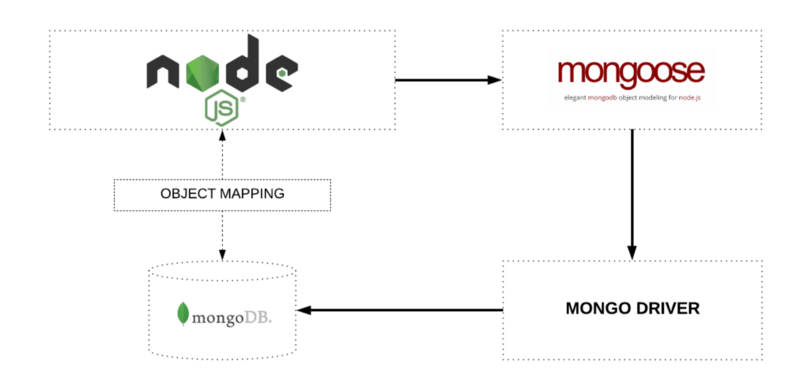
\includegraphics[width=\linewidth]{res/Mongoose.png}
  \caption[Mappatura di oggetti tra Node e MongoDB tramite Mongoose.]{Mappatura di oggetti tra Node e MongoDB tramite Mongoose.\protect\cite{freecodecamp}}
  \label{fig:Mongoose}
\end{figure}

La chiamata \code{require("mongoose")} restituisce un oggetto Singleton, così come avviene per qualsiasi modulo importato in ES6. Ciò significa che alla prima chiamata verrà creata e restituita un'istanza della classe \texttt{Mongoose}, e alle chiamate successive verrà restituita la stessa istanza creata precedentemente e restituita la prima volta.\cite{freecodecamp}

Uno schema descrive il costrutto dei dati di un documento, ovvero definisce il nome e il tipo di ciascun elemento. È ragionevole associare uno schema a ciascuna collezione presente nel database. Un esempio di schema in Mongoose è il seguente:

\begin{lstlisting}
var userSchema = new mongoose.Schema({
 name: String,
 email: String,
 createdOn: Date,
 verified: Boolean
});
\end{lstlisting}

Un altro elemento chiave di Mongoose è il cosiddetto modello. Esso è la versione compilata dello schema; un'istanza del modello verrà mappata a un documento nel database. Si occupa di gestire la lettura, la creazione, l'aggiornamento e la cancellazione dei documenti.\cite{holmes}
\begin{lstlisting}
var User = mongoose.model("User", userSchema);
\end{lstlisting}

Le specifiche di connessione tra Mongoose e il database sono contenute nella cosiddetta stringa di connessione, espressa nel seguente formato:\cite{connection-string}
\begin{lstlisting}
mongodb://[username:password@]host1[:port1][,...hostN[:portN]][/[database][?opzioni]]
\end{lstlisting}

Vi sono due metodi per effettuare la connessione al database con Mongoose: \texttt{mongoose.connect} e \code{createConnection}.\cite{holmes-connection}

Il primo imposta la connessione di default, la quale sarà accessibile da qualsiasi punto dell'applicazione se impostata correttamente.
\begin{lstlisting}
var dbURI = "mongodb://localhost/mydatabase";
mongoose.connect(dbURI);
\end{lstlisting}
Il secondo viene utilizzato nel caso sia necessario stabilire più di una connessione, che sia allo stesso database che a un altro.
\begin{lstlisting}
var dbURI = "mongodb://localhost/myadmindatabase";
var adminConnection = mongoose.createConnection(dbURI);
\end{lstlisting}

\subsection{Stardog}
Il focus principale di Stardog è la costruzione di Enterprise Knowledge Graph, attraverso cui è possibile visualizzare informazioni e relazioni da molteplici sorgenti di dati eterogenee e rendere i dati accessibili all'interogazione e manipolazione. 
Per enterprise knowledge graph si intende 

A differenza di un database a grafo pensato unicamente per l'archiviazione dei dati, una piattaforma Enterprise Knowledge Graph ha anche funzionalità che supportano la rappresentazione della conoscenza nel grafo e consentono, tra le altre cose, la comprensione da parte della macchina. Ad esempio, mentre un database a grafo sa che esiste un'interrelazione tra un nodo persona nel database A e un nodo organizzazione nel database B, un Enterprise Knowledge Graph comprende anche la natura di tale interrelazione. 

È una raccolta di riferimenti alle risorse di conoscenza, ai contenuti e ai dati della tua organizzazione che sfrutta un modello di dati per descrivere le persone, i luoghi e le cose e il modo in cui sono correlati.

Stardog permette l'interrogazione con query SPARQL mediante linea di comando SSH o richieste HTTP. È possibile utilizzare l'editor Stardog Studio per importare, visualizzare e interrogare ontologie OWL salvate in Stardog; non è supportata tuttavia la modellazione di ontologie, possibile nel tool Protegé. 

È possibile effettuare path query, ovvero ottenere come output l'insieme di archi che legano due nodi del grafo\cite{stardog}.

\subsection{Textract}
\textbf{Textract} è una libreria Python atta all'estrazione del testo da un file. Supporta l'estrazione da file di diversi formati comuni appoggiandosi a parser dedicati.

Una volta invocato, il metodo \texttt{texttract.process('path/to/file.extension')} instrada il nome del file al parser appropriato e restituisce il testo estratto come stringa di byte codificata con la codifica specificata.\cite{textract}

\subsection{Tesseract}
\textbf{Tesseract} è un motore di riconoscimento ottico dei caratteri OCR sviluppato dalla Hewlett-Packard tra il 1985 e il 1995; è stato abbandonato a se stesso per i successivi 10 anni, fino a quando nel 2005 ne è stato rilasciato il codice
sorgente con una licenza libera. Dal 2006 a novembre 2018 è stato sviluppato da Google.

È considerato uno dei più accurati motori OCR attualmente disponibili, con il vantaggio, non indifferente, che essendo free software è accessibile e utilizzabile da tutti.
Supporta la codifica Unicode (UTF-8), può riconoscere oltre 100 lingue.

Tesseract 4 aggiunge un nuovo motore OCR basato sulla rete neurale (LSTM) che si concentra sul riconoscimento della linea, ma supporta anche il motore OCR Tesseract legacy di Tesseract 3 che funziona riconoscendo i modelli di caratteri.

\subsubsection{Python-tesseract}
\textbf{Python-tesseract} è un wrapper per il motore Tesseract-OCR di Google. È utile come script di invocazione autonomo per tesseract, poiché può leggere tutti i tipi di immagine supportati dalle librerie di immagini Pillow e Leptonica, inclusi jpeg, png, gif, bmp, tiff e altri. Inoltre, se usato come script, Python-tesseract stamperà il testo riconosciuto invece di scriverlo su un file.

\subsection{PDFMiner}
\textbf{PDFMiner} è una libreria per l’analisi di documenti PDF scritta in Python. Oltre al testo, estrae anche le posizioni corrispondenti, i nomi dei caratteri, le dimensioni dei caratteri, la direzione di scrittura (orizzontale o verticale) per ciascun segmento di testo. Non riconosce il testo nelle immagini.

PDFMiner si basa sulla ricostruzione di alcune delle informazioni contenute nel formato PDF, adottando una strategia di parsing lazy, cioè quella di analizzare le istruzioni della struttura del documento PDF solo quando è necessario.
Per effettuare il parsing è necessario utilizzare almeno le classi \texttt{PDFParser}, che si occupa di recuperare i dati dal file, e \texttt{PDFDocument}, che si occupa di memorizzare i dati recuperati.
Per elaborare il contenuto della pagine viene utilizzata la classe \texttt{PDFPageInterpreter}. \texttt{PDFDevice} converte il contenuto in formati diversi. \texttt{PDFResourceManager} viene utilizzato per archiviare risorse condivise come caratteri o immagini.